
\documentclass{standalone}
\usepackage{tikz}
\usepackage{standalone}
\usetikzlibrary{calc}
\begin{document}
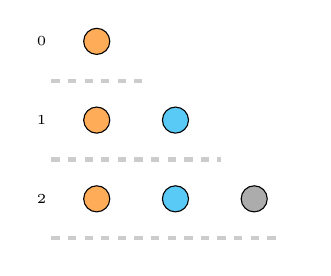
\begin{tikzpicture}
\node[circle, draw=black, draw=black, fill=orange!65] (0) at (0, 0) {};
\node[circle, draw=black, draw=black, fill=cyan!65] (1) at (1, 0) {};
\node[circle, draw=black, fill=gray!65]  (2) at (2, 0) {};
\node[circle, draw=black, draw=black, fill=orange!65] (3) at (0, 1) {};
\node[circle, draw=black, draw=black, fill=cyan!65] (4) at (1, 1) {};
\node[circle, draw=black, draw=black, fill=orange!65] (5) at (0, 2) {};

\node (l0) at (-.7, 2) {\tiny{0}};
\node (l0) at (-.7, 1.5) {};
\node (l1) at (0.7, 1.5) {};
\draw[line width=1.5pt, dashed, -, black!20] (l0) -- (l1);

\node (l0) at (-.7, 1) {\tiny{1}};
\node (l0) at (-.7, 0.5) {};
\node (l1) at (1.7, 0.5) {};
\draw[line width=1.5pt, dashed, -, black!20] (l0) -- (l1);

\node (l0) at (-.7, 0) {\tiny{2}};
\node (l0) at (-.7, -.5) {};
\node (l1) at (2.5, -.5) {};
\draw[line width=1.5pt, dashed, -, black!20] (l0) -- (l1);
                \end{tikzpicture}
                \end{document}